\paragraph{add\_many\_u32}

\hspace*{\fill}

\indent U32AddManyGate is a gate to perform addition on num\_addends different 32-bit values, plus a small carry. 
There can be up to 16 operations per gate.

The gate structure is like \figref{fig:add-many-u32}.

\begin{figure}[!ht]
    \centering
    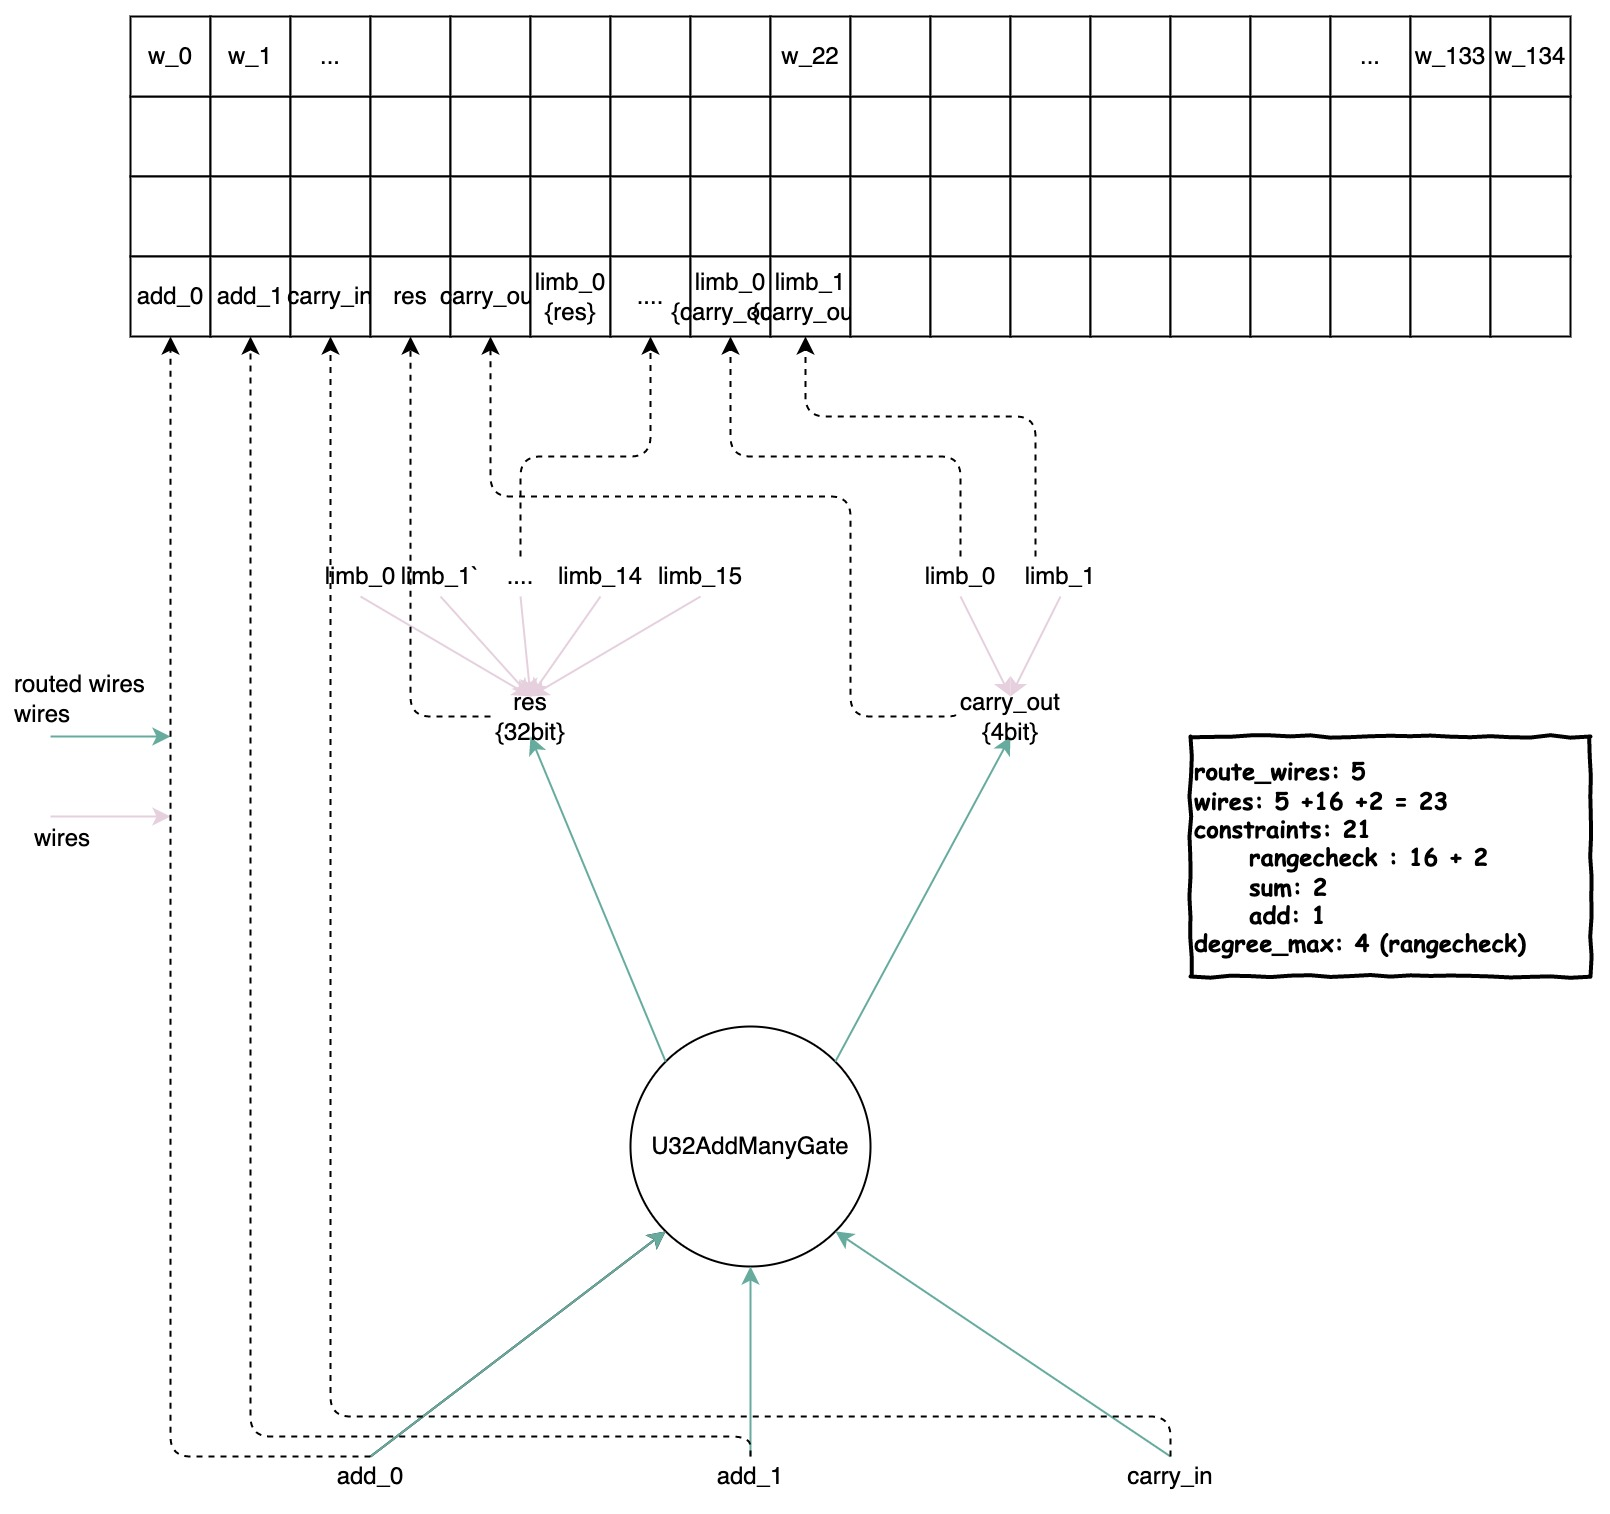
\includegraphics[width=0.6\textwidth]{gates/add_many_u32.jpeg}
    \caption{U32AddManyGate}
    \label{fig:add-many-u32}
\end{figure}

Constraints for each operation:
\begin{itemize}
    \item Constrain the result of addends summation equals results of res and carry\_out calculation. -- 1 constraint with degree 1
    \begin{lstlisting}[language=rust]
let base = F::Extension::from_canonical_u64(1 << 32u64);
let combined_output = output_carry * base + output_result;
constraints.push(combined_output - computed_output);
    \end{lstlisting}
    \item Limbs range check. -- 18(limbs) constraints with degree 4.(limbs are all 2-bits)
    \begin{lstlisting}[language=rust]
let product = (0..max_limb)
    .map(|x| this_limb - F::Extension::from_canonical_usize(x))
    .product();
constraints.push(product);
    \end{lstlisting}
    \item Constrain limbs for res and carry\_out. -- 2 constraints with degree 1.
\end{itemize}

In summary, there are 21 constraints for each operation. The degree of the gate is 4 which is needed by the 4-bits limbs range check.
